% ------------------------------------------------------------------
\renewcommand{\thisweek}{MATH327 Week 6}
\renewcommand{\moddate}{Last modified 7 Mar.~2021}
\setcounter{section}{6}
\setcounter{subsection}{0}
\phantomsection
\addcontentsline{toc}{section}{Week 6: Grand-canonical ensemble}
\section*{Week 6: Grand-canonical ensemble}
\subsection{The particle reservoir and chemical potential}
This week we define and develop the third and final statistical ensemble to be studied in this module, which is known as the grand-canonical ensemble.
Our approach will follow the pattern set by our previous development of the canonical ensemble.
Recall that statistical ensembles are probability spaces describing the micro-states that a system can adopt as it evolves in time, subject to certain constraints.
We began in week 2 with the micro-canonical ensemble, in which these constraints were conservation of the internal energy $E$ and particle number $N$.
We then introduced the canonical ensemble in week 3 by allowing the system's internal energy to fluctuate, while keeping its temperature $T$ fixed through thermal contact with a large external thermal reservoir.

The next step is to allow \textit{both} the system's energy and its particle number to fluctuate.
In the same way as for the canonical ensemble, we allow energy exchange with a large thermal reservoir that fixes the temperature $T$.
In addition, we now allow the system to exchange particles with a large external \textit{particle reservoir}.
Typically the system's surroundings will simultaneously serve as both thermal and particle reservoir.

By analogy with the temperature held fixed by the thermal reservoir, we expect there to be some quantity that this particle reservoir will hold fixed.
Recall that we initially defined the temperature in the context of the micro-canonical ensemble in thermodynamic equilibrium (\eq{eq:temperature}), as the dependence of the entropy on the internal energy for a fixed number of degrees of freedom:
\begin{equation*}
  \frac{1}{T} = \left. \pderiv{S}{E}\right|_N.
\end{equation*}
The quantity we are now interested in comes from the complementary analysis interchanging the roles of $E$ and $N$.

\begin{shaded}
  In thermodynamic equilibrium, the \textbf{chemical potential} in the micro-canonical ensemble is defined by
  \begin{equation}
    \label{eq:chem_pot}
    \mu = -T \left. \pderiv{S}{N}\right|_E.
  \end{equation}
\end{shaded}

This definition is not terribly intuitive, nor is the chemical potential a familiar concept from everyday experiences.
To gain some insight into the chemical potential, we can note (from either \eq{eq:temperature} or \eq{eq:first_law}) that $\mu$ has dimensions of energy.
We can also expect the partial derivative $\pderiv{S}{N}$ to be positive in general, since systems with more degrees of freedom generically have more entropy corresponding to the greater amount of information they can contain.
This can be checked explicitly for the spin system (\eq{eq:dist_entropy}) and ideal gas (\eq{eq:ideal_entropy}) we previously analyzed.
The choice of sign in \eq{eq:chem_pot} therefore means that we should expect the chemical potential to be negative, in `natural' systems with positive temperatures.

The motivation for this negative sign comes from considering a net flow of particles between two systems with the same temperature $T$ but different $\pderiv{S}{N}$.
According to the second law of thermodynamics, the system with the larger $\pderiv{S}{N}$ will gain particles, so that the amount of entropy it gains will be greater than the amount lost by the system with the smaller $\pderiv{S}{N}$.
In other words, we expect particles to flow from systems with larger (less-negative) $\mu$ to systems with smaller (more-negative) $\mu$, which provides an intuitive analogue to heat flowing from systems with larger $T$ to those with smaller $T$.

\begin{shaded}
  We are now able to define a \textbf{grand-canonical ensemble} to be a statistical ensemble characterized by its fixed temperature $T$ and fixed chemical potential $\mu$, with the temperature held fixed through contact with a thermal reservoir and the chemical potential held fixed through contact with particle reservoir.
\end{shaded}
% ------------------------------------------------------------------



% ------------------------------------------------------------------
\subsection{The grand-canonical partition function}


\begin{center}
  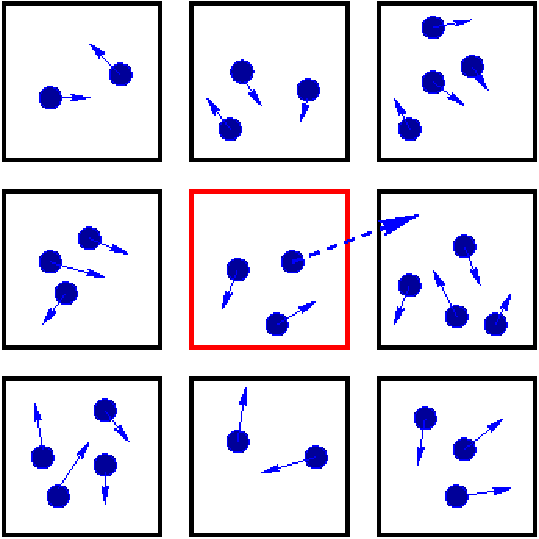
\includegraphics[width=0.7\textwidth]{figs/week06_reservoir.pdf}
\end{center}

\TODO{Being written...}
% ------------------------------------------------------------------



% ------------------------------------------------------------------
\newpage % TODO: Placeholder...
\subsection{The grand-canonical potential}
\TODO{$\Phi$ rather than $\Om$...}
\TODO{Being written...}
% TODO: Fugacity expansion?
% ------------------------------------------------------------------
